\section{经验平均的应用}
\label{sec:lln-applications}

实际计算中出现的许多量都是平均：一个事件发生的频率、一个函数在观测上的平均、样本的各阶矩。要对它们用大数律，先把它们写成某列随机变量的样本平均，再逐项核对三件事：这列变量是否独立同分布，被平均的函数是否在看到数据之前就已固定，它的期望是否绝对可积。

设$X_1,X_2,\dots$独立同分布，取值于集合$\mathcal{X}$（例如$\mathbb{R}$或$\mathbb{R}^d$），共同分布为$P_X$。本节只讨论预先给定的事件和函数；在看到数据之后再挑选函数或事件，需要对一整族同时成立的保证，那是统计推断的问题。

\subsection{事件频率}
\label{sec:lln-frequency}

第~\ref{chap:classical-probability}章用重复试验中的相对频率解释概率，并在模拟中看到频率稳定在概率附近。现在可以说明它为什么稳定。

对固定的事件$A\subseteq\mathcal{X}$（要求$A$是可测集，即$\{X_1\in A\}$是事件），令
\begin{equation}
 f_n(A)=\frac{1}{n}\sum_{i=1}^{n}\mathbf{1}_{A}(X_i) ,
 \label{eq:lln-frequency}
\end{equation}
即前$n$次观测中落入$A$的比例。示性变量$\mathbf{1}_A(X_i)$独立同分布，服从$\operatorname{Bern}(p)$，其中$p=\mathbb{P}(X_1\in A)$。它们取值于$\{0,1\}$，均值为$p$，方差为$p(1-p)$。

\begin{theorem}[频率的大数律]
\label{thm:lln-frequency}
设$X_1,X_2,\dots$独立同分布，$A$是固定的可测集，$p=\mathbb{P}(X_1\in A)$。则$f_n(A)\xrightarrow{\mathrm{a.s.}}p$，并且对每个$\varepsilon>0$与每个$n$，
\begin{equation}
 \mathbb{P}\bigl(\lvert f_n(A)-p\rvert\geq\varepsilon\bigr)\leq\frac{p(1-p)}{n\varepsilon^2}\leq\frac{1}{4n\varepsilon^2} .
 \label{eq:lln-frequency-bound}
\end{equation}
\end{theorem}

\begin{proof}
示性变量有界，从而可积且方差有限。对它们用定理~\ref{thm:lln-slln}得到几乎必然收敛，用定理~\ref{thm:lln-wlln-variance}得到第一个不等式。第二个不等式来自$p(1-p)\leq1/4$。
\end{proof}

这个结论称为Borel强大数律，它是概率的频率解释的数学内容。以骰子为例，令$A$为“掷出$6$点”，则几乎每一串掷骰记录中$6$点的比例都趋于$1/6$。这里的“几乎每一串”有确切含义：例外的记录（例如永远掷出$6$点）当然可以写下来，但它们的全体概率为零。

\paragraph{随机投点估面积}
频率还可以用来计算面积。设$U,V$独立且都服从$\operatorname{Unif}(0,1)$，事件$A=\{U^2+V^2\leq1\}$是单位正方形中的四分之一圆盘，概率等于它的面积$\pi/4$。在正方形中独立投点，落入圆盘的比例几乎必然趋于$\pi/4$，所以$4f_n(A)\to\pi$。这种用随机样本的平均计算积分的方法称为Monte Carlo方法。

图~\ref{fig:lln-monte-carlo}(a)画出一次投点（种子$31$）的前$400$个点，其中$316$个落在圆内，给出估计$4\times316/400=3.16$。图(b)画出五次独立投点的估计路径，$n=10^4$时它们落在$3.130$到$3.156$之间。式~\eqref{eq:lln-frequency-bound}给出估计的标准差
\[
 4\sqrt{\frac{p(1-p)}{n}}=4\sqrt{\frac{0.7854\times0.2146}{10^4}}\approx0.016 ,
\]
与五个估计的散布相符。误差怎样随样本数缩小、怎样减小它，是第~\ref{chap:monte-carlo-integration-error}章与第~\ref{chap:variance-reduction}章的内容。

\begin{BookInlineFigure}
 \centering
 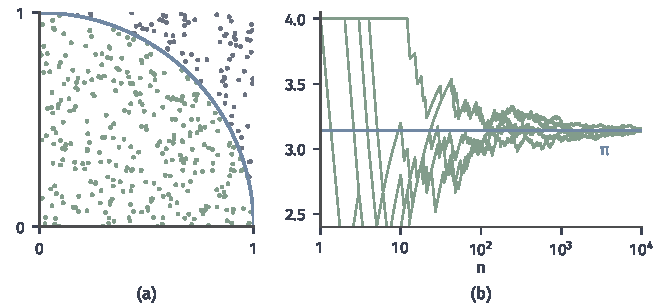
\includegraphics[width=112mm]{figures/07-probability/03-probability-limits/matplotlib/lln-monte-carlo/figure.pdf}
 \caption{用频率估计四分之一圆的面积。(a)单位正方形中的前$400$个均匀点（种子$31$），绿点落在四分之一圆内，灰点落在圆外，蓝线为圆弧；(b)五次独立投点（种子$31$至$35$）的估计$4f_n(A)$（绿线）与$\pi$（蓝线），横轴为对数刻度。}
 \label{fig:lln-monte-carlo}
\end{BookInlineFigure}

\paragraph{固定事件与事件族}
定理~\ref{thm:lln-frequency}对每个固定的$A$给出一个概率为一的事件$\Omega_A$，在其上$f_n(A)\to p$。不同的$A$对应的例外集不同。对可数个事件$A_1,A_2,\dots$，可数个零概率集的并仍是零概率集，所以几乎必然地，$f_n(A_j)\to\mathbb{P}(X_1\in A_j)$对所有$j$同时成立。例如所有端点为有理数的区间可以同时处理。

对所有事件同时成立却是错的。设$X_i$服从$\operatorname{Unif}(0,1)$，取事件$A=\{X_1,\dots,X_n\}$，即观测到的那些点组成的有限集。它的频率是$f_n(A)=1$，概率却是$\mathbb{P}(X_1\in A)=0$，因为连续分布不给单点任何质量。图~\ref{fig:lln-finite-event}画出了这种情形。于是对每个$n$和每个样本点，
\[
 \sup_{A}\bigl\lvert f_n(A)-\mathbb{P}(X_1\in A)\bigr\rvert=1 .
\]

\begin{BookInlineFigure}
 \centering
 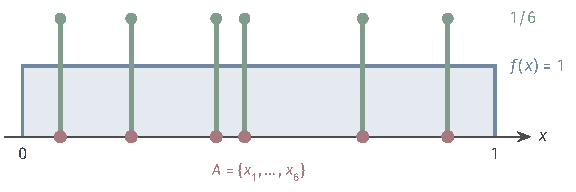
\includegraphics[width=98mm]{figures/07-probability/03-probability-limits/tikz/lln-finite-event/figure.pdf}
 \caption{均匀分布（蓝色，密度为$1$）与六个观测点的经验质量（绿色竖线，每点$1/6$）。由观测点组成的事件$A=\{x_1,\dots,x_6\}$（红点）频率为$1$，在均匀分布下的概率为$0$。}
 \label{fig:lln-finite-event}
\end{BookInlineFigure}

问题出在事件依赖于数据。定理中的$A$必须在观测之前固定。对半直线$(-\infty,t]$这样的特殊事件族，频率可以对整族一致收敛，但那需要额外的论证，属于统计推断的内容，见\BookChapterRef{chap:nonparametric-inference}{卷八第2章“非参数分布与函数推断”}。

\subsection{函数平均与样本矩}
\label{sec:lln-function-averages}

频率是函数平均的特例：被平均的函数是示性函数。一般地，取一个固定的函数$g\colon\mathcal{X}\to\mathbb{R}$（要求可测，使$g(X_1)$是随机变量），考虑$\frac1n\sum_{i\leq n}g(X_i)$。

\begin{theorem}[函数平均的大数律]
\label{thm:lln-function-average}
设$X_1,X_2,\dots$独立同分布，$g$可测，$\mathbb{E}[\lvert g(X_1)\rvert]<\infty$。则
\begin{equation}
 \frac{1}{n}\sum_{i=1}^{n}g(X_i)\xrightarrow{\mathrm{a.s.}}\mathbb{E}[g(X_1)] .
 \label{eq:lln-function-average}
\end{equation}
\end{theorem}

\begin{proof}
$g(X_1),g(X_2),\dots$是独立变量的函数，所以相互独立；它们的分布都是$g(X_1)$的分布，所以同分布。由假设它们可积，对它们用定理~\ref{thm:lln-slln}即可。
\end{proof}

条件$\mathbb{E}[\lvert g(X_1)\rvert]<\infty$必须针对$g(X_1)$检查，而不是针对$X_1$。例如$X_1\sim\operatorname{Unif}(0,1)$有界，但$g(x)=1/x$使
\[
 \mathbb{E}[g(X_1)]=\int_0^1\frac{\mathrm{d}x}{x}=\infty ,
\]
定理不能直接使用。这时平均$\frac1n\sum_i1/X_i$几乎必然趋于$+\infty$：对每个$M>0$，$1/X_i\geq\min\{1/X_i,M\}$，后者有界，由定理得
\[
 \liminf_{n\to\infty}\frac1n\sum_{i=1}^{n}\frac{1}{X_i}\geq\mathbb{E}\bigl[\min\{1/X_1,M\}\bigr]\quad\text{几乎必然},
\]
而右边随$M\to\infty$单调增至$\infty$。取$M=1,2,\dots$，可数个例外集的并仍是零概率集。

\paragraph{样本矩}
取$g(x)=x^r$，$r$为正整数，得到$r$阶\term{样本矩}（sample moment）
\[
 m_{n,r}=\frac{1}{n}\sum_{i=1}^{n}X_i^r .
\]
由定理~\ref{thm:lln-function-average}，只要$\mathbb{E}[\lvert X_1\rvert^r]<\infty$，就有$m_{n,r}\to\mathbb{E}[X_1^r]$几乎必然成立。一阶样本矩就是样本平均$\bar{X}_n$。

\paragraph{样本方差}
常用的\term{样本方差}（sample variance）是
\begin{equation}
 S_n^{2}=\frac{1}{n-1}\sum_{i=1}^{n}\bigl(X_i-\bar{X}_n\bigr)^2,\qquad n\geq2 .
 \label{eq:lln-sample-variance}
\end{equation}
这里$S_n^2$是一个新记号，与部分和$S_n$的平方无关；本小节只在这个意义下使用它。它不是单个函数的平均，因为每一项都含有$\bar{X}_n$。先把平方和展开，用$\sum_iX_i=n\bar{X}_n$，
\[
 \sum_{i=1}^{n}(X_i-\bar{X}_n)^2=\sum_{i=1}^{n}X_i^2-2\bar{X}_n\sum_{i=1}^{n}X_i+n\bar{X}_n^2=\sum_{i=1}^{n}X_i^2-n\bar{X}_n^2 .
\]
于是样本方差写成两个样本矩的组合：
\[
 S_n^{2}=\frac{n}{n-1}\bigl(m_{n,2}-\bar{X}_n^2\bigr) .
\]

现在只需$\mathbb{E}[X_1^2]<\infty$。这时$X_1$也可积，由定理~\ref{thm:lln-function-average}，$m_{n,2}\to\mathbb{E}[X_1^2]$与$\bar{X}_n\to\mu$各在一个概率为一的事件上成立。在两个事件的交上，平方与乘积都是连续运算，$n/(n-1)\to1$，所以
\begin{equation}
 S_n^{2}\xrightarrow{\mathrm{a.s.}}\mathbb{E}[X_1^2]-\mu^2=\sigma^2 .
 \label{eq:lln-sample-variance-limit}
\end{equation}

这个结论只用到有限的二阶矩，不需要假设四阶矩有限。四阶矩控制的是$S_n^2$本身的方差，也就是它在$\sigma^2$附近波动的大小；收敛本身不需要它。

用一组具体数据核对公式。掷五次骰子得到$2,5,3,6,1$，则
\[
 \bar{X}_5=\frac{17}{5}=3.4,\qquad m_{5,2}=\frac{4+25+9+36+1}{5}=15 ,
\]
所以
\[
 S_5^2=\frac54\bigl(15-3.4^2\bigr)=\frac54\times3.44=4.3 .
\]
五次观测太少，$4.3$离$\sigma^2=35/12\approx2.917$还很远。图~\ref{fig:lln-sample-variance}(a)是五条长路径（种子$41$），$n=10^5$时样本方差落在$2.903$到$2.924$之间。

图(b)换成自由度$\nu=3$的t分布（种子$42$）。它的方差为$\nu/(\nu-2)=3$，四阶矩却是无穷。样本方差仍然收敛到$3$，但路径不时被一个大观测猛地推高，再慢慢回落，收敛明显比骰子慢。这正说明四阶矩影响的是波动大小，而不是收敛与否。

\begin{BookInlineFigure}
 \centering
 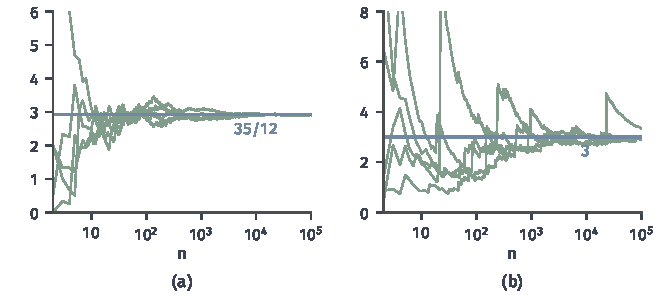
\includegraphics[width=112mm]{figures/07-probability/03-probability-limits/matplotlib/lln-sample-variance/figure.pdf}
 \caption{样本方差$S_n^2$的路径，每图五条（绿线），横轴为对数刻度，蓝线为总体方差。(a)均匀骰子（种子$41$），$\sigma^2=35/12$；(b)自由度$3$的t分布（种子$42$），$\sigma^2=3$，四阶矩无穷。}
 \label{fig:lln-sample-variance}
\end{BookInlineFigure}

\paragraph{适用边界}
本节的结论说明：给定分布与给定函数，经验平均几乎必然趋于相应的期望。它不回答平均以多快的速度接近期望，也不回答在平均附近放大后的误差服从什么分布；前者需要矩或尾部信息，后者是中心极限定理的内容。用样本平均去估计未知的期望、给出可信区间，则是统计推断的问题，由卷八承担。
